\subsection{極低温連続回転式半波長板 (HWP)}
\label{sec:HWP}
大気による熱放射は常に揺らいでいる。
これは大気による $1/f$ ノイズとして知られ、CMB偏光観測実験においては、このノイズとCMB偏光信号を分離することが重要である。
SATでは、この大気による熱放射を取り除くために、極低温連続回転式半波長板(cryogenic continuously rotating Half-Wave Plate, 以後、単にHWPと呼ぶ)を用いる~\cite{so:hwp_yamada}。

一般に、HWPは複屈折の特性を持つ素材からなり、素子中のある決まった軸(光軸)に対して電場成分を反転させる光学素子である。
この光軸を1軸とし、光軸に対して垂直なHWP平面上の軸を2軸と定める。
今、$xyz$ 直交座標系を考え、$z$ 軸正の方向に進む光を考える。その複素電場 $\bm{\mathcal{E}}$ は一般に
\begin{equation}
    \bm{\mathcal{E}} = \mathcal{E}_{x}\bm{\hat{e}}_{x} + \mathcal{E}_{y}\bm{\hat{e}}_{y}
\end{equation}
と表される。
初めに、$x$ 軸と1軸が一致し、$y$ 軸が2軸と一致するような場合を考える。この時、電場 $\bm{\mathcal{E}}$ がHWPを通過することで
\begin{align}
    \mathcal{E}_{x} &= \mathcal{E}_{x} \\
    \mathcal{E}_{y} &= -\mathcal{E}_{y}
\end{align}
となる。1軸($x$軸)に対して電場成分が反転している。
これにより、1軸に対して $\chi$ だけ傾いて直線偏光している入射光は、$-\chi$ だけ傾いて直線偏光した光に変換される(図\ref{fig:so-hwp_satoru})。
入射してくる光のストークスパラメータを $I_{\mathrm{in}},\,Q_{\mathrm{in}},\,U_{\mathrm{in}},\,V_{\mathrm{in}}$ とすると、
HWPを通過した後の光のストークスパラメータ $I_{\mathrm{out}},\,Q_{\mathrm{out}},\,U_{\mathrm{out}},\,V_{\mathrm{out}}$ は
式\eqref{eq:stokes_I_complex}$\sim$\eqref{eq:stokes_V_complex}を用いて
\begin{equation}
    \mqty(I_{\mathrm{\mathrm{out}}} \\
          Q_{\mathrm{\mathrm{out}}} \\
          U_{\mathrm{\mathrm{out}}} \\
          V_{\mathrm{\mathrm{out}}}
    ) = 
    \mqty(1 & 0 & 0 & 0 \\ 
          0 & 1 & 0 & 0 \\
          0 & 0 & -1 & 0 \\
          0 & 0 & 0 & -1
          )
    \mqty(I_{\mathrm{in}} \\
          Q_{\mathrm{in}} \\
          U_{\mathrm{in}} \\
          V_{\mathrm{in}}
          )
\end{equation}
と計算でき、$Q,\,U$ を反転させることがわかる。
HWPが行うストークスパラメータの変換行列 $M_{\mathrm{HWP}}$ を
\begin{equation}
    M_{\mathrm{HWP}} = 
    \mqty(1 & 0 & 0 & 0 \\ 
          0 & 1 & 0 & 0 \\
          0 & 0 & -1 & 0 \\
          0 & 0 & 0 & -1
          )
\end{equation}
と定義する。

\begin{figure}[H]
    \centering
    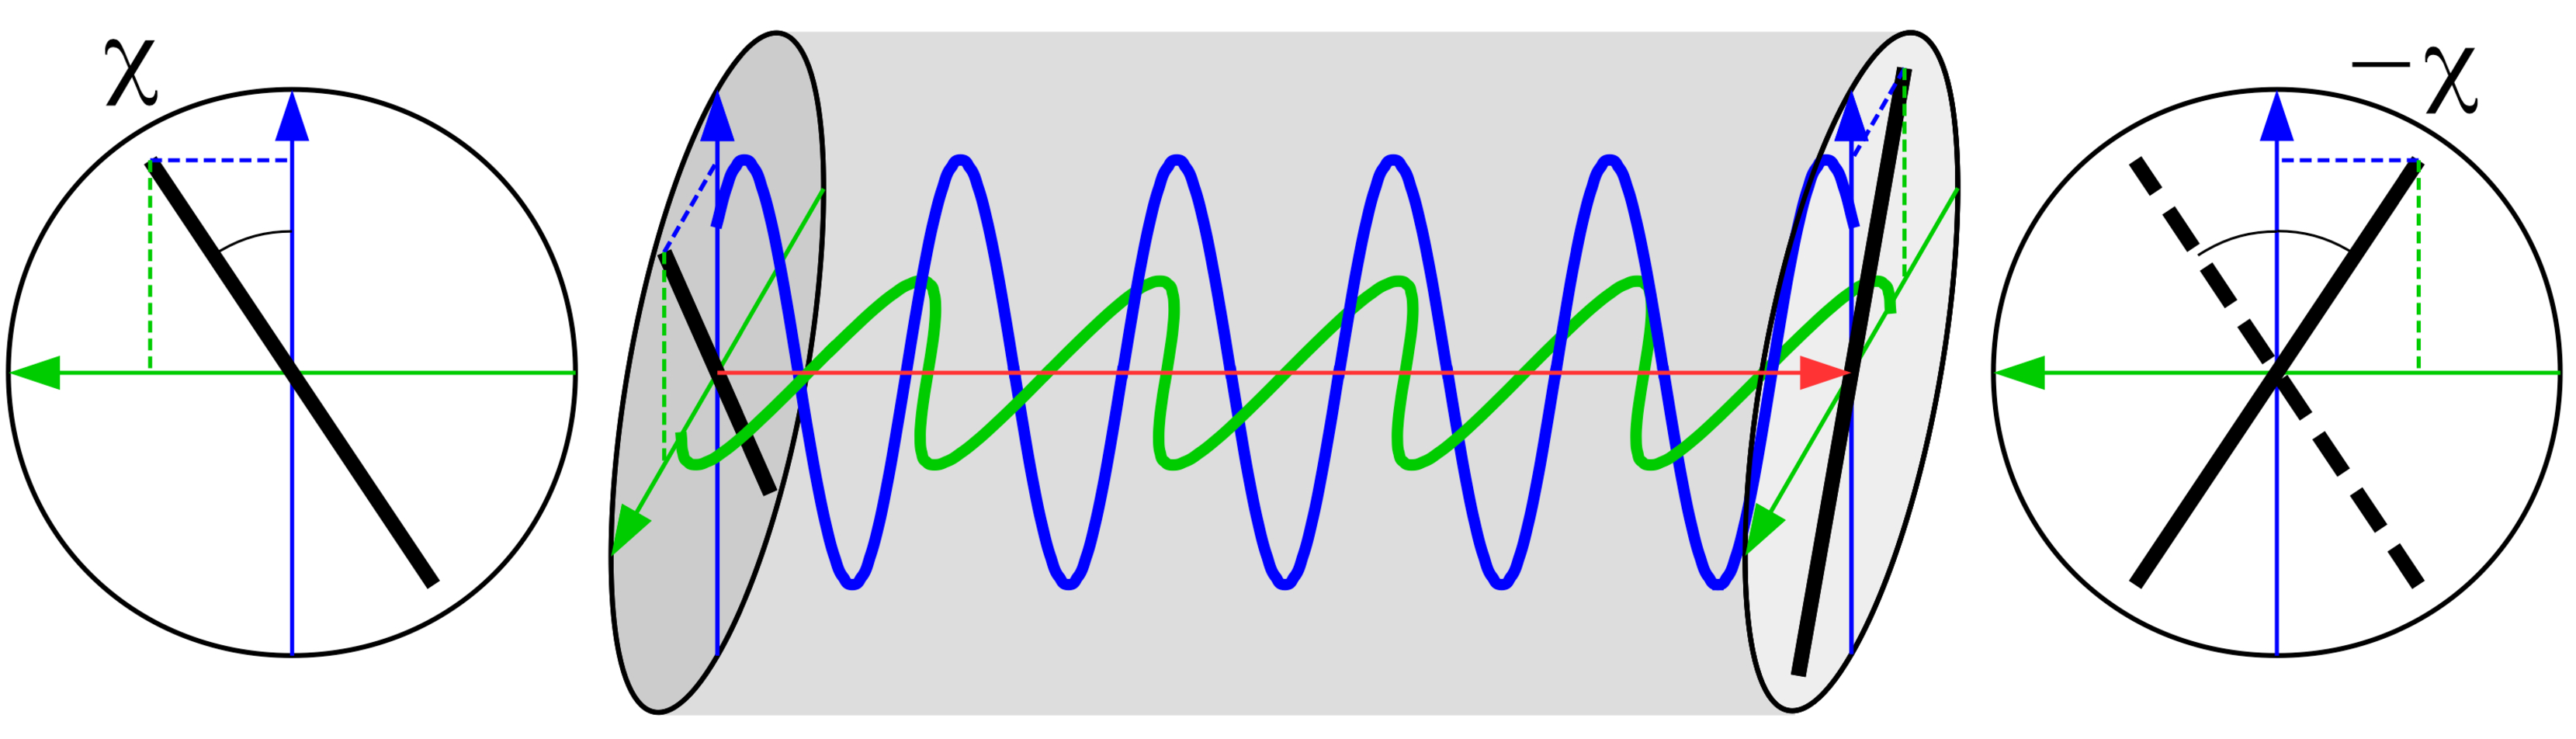
\includegraphics[width=0.8\textwidth]{simons_observatory/hwp_satoru.pdf}
    \caption{HWPを通過することで、偏光角が変化することを示した概念図~\cite{takakura_PhD}。青い軸が1軸、緑の軸が2軸に対応する。
    入射した直線偏光の偏光角が1軸に対して $\chi$ であり、複屈折によって $-2\chi$ だけ変化する。}
    \label{fig:so-hwp_satoru}
\end{figure}

次に、HWPの1軸が $x$ 軸から測って $\theta_{\mathrm{HWP}}$ だけ回転しているような場合を考える(図\ref{})。
入射光のストークスパラメータを測る基底を $x,\,y$ 軸から 1,\,2軸に変換したあと、
$U,\,V$ を反転、基底をもとに戻すという操作を行えば、HWPを通過した後の光のストークスパラメータを計算できる。
そこで、座標を $\theta$ だけ回転したときのストークスパラメータの変換行列を $R(\theta)$ とすると、式\ref{eq:stokes_transform}より
\begin{equation}
    R_{\theta} = 
    \mqty(1 & 0 & 0 & 0 \\ 
          0 & \cos 2\theta  & \sin 2\theta & 0 \\
          0 & -\sin 2\theta & \cos 2\theta & 0 \\
          0 & 0 & 0 & 1
          )
\end{equation}
である。この行列を用いて、HWPを通過した後の光のストークスパラメータは
\begin{equation}
    \mqty(I_{\mathrm{\mathrm{out}}} \\
          Q_{\mathrm{\mathrm{out}}} \\
          U_{\mathrm{\mathrm{out}}} \\
          V_{\mathrm{\mathrm{out}}}
    ) = 
    R\qty(-\theta_{\mathrm{HWP}}) M_{\mathrm{HWP}} R\qty(\theta_{\mathrm{HWP}})
    \mqty(I_{\mathrm{in}} \\
          Q_{\mathrm{in}} \\
          U_{\mathrm{in}} \\
          V_{\mathrm{in}}
          )
\end{equation}
となる。
この性質により、入力信号のストークスパラメータがそれぞれ $I_{\mathrm{in}}(t), Q_{\mathrm{in}}(t), U_{\mathrm{in}}(t)$ であるとき、出力信号 $d_m(t)$ は
\begin{equation}
    d_{\mathrm{m}}(t) = I_{\mathrm{in}}(t) + \varepsilon\Re\qty[\qty(Q_{\mathrm{in}}(t)+iU_{\mathrm{in}}(t))\exp(-i 4\chi)]
\end{equation}
となる。ここで、$\varepsilon$ は変調効率である。SOでは、HWPを $2\ \mathrm{Hz}$ で回転させることで、連続的に入射する直線偏光による信号を $8\ \mathrm{Hz}$ に変調して出力する。
HWPの角振動数を $\omega_{\mathrm{HWP}}$ とし、初期位相を $\chi_0$ とすると、$\chi(t) = \omega_{\mathrm{HWP}}t + \chi_{0}$ と表され、出力信号は
\begin{equation}
    d_{\mathrm{m}}(t) = I_{\mathrm{in}}(t) + \varepsilon\Re\qty[\qty(Q_{\mathrm{in}}(t)+iU_{\mathrm{in}}(t))\exp(-i \qty(4\omega_{\mathrm{HWP}}t + 4\chi_0))]
\end{equation}
となる。検出器はある偏光角方向 $\theta_{\mathrm{det}}$ にのみ感度を持つため、最終的に検出器が読み出す信号 $d_{\mathrm{m}, \mathrm{det}}$ は
\begin{equation}
    \label{eq:so-hwp_modulation}
    d_{\mathrm{m}, \mathrm{det}}(t) = I_{\mathrm{in}}(t) + \varepsilon\Re\qty[\qty(Q_{\mathrm{in}}(t)+iU_{\mathrm{in}}(t))\exp\qty{-i \qty(4\omega_{\mathrm{HWP}}t + 4\chi_0 - 2\theta_{\mathrm{det}})}]
\end{equation}
となる。この信号のフーリエ変換は
\begin{equation}
    \begin{split}
        \tilde{d}_{\mathrm{m}, \mathrm{det}}(\Omega) = &\tilde{I}_{\mathrm{in}}(\Omega) \\
            &+ \dfrac{\varepsilon}{2}\qty[\qty{\tilde{Q}_{\mathrm{in}}(\Omega+4\omega_{\mathrm{HWP}})+i\tilde{U}_{\mathrm{in}}(\Omega+4\omega_{\mathrm{HWP}})}\exp\qty{-i\qty(4\chi_0 - 2\theta_{\mathrm{det}})}] \\
            &+ \dfrac{\varepsilon}{2}\qty[\qty{\tilde{Q}_{\mathrm{in}}(\Omega-4\omega_{\mathrm{HWP}})-i\tilde{U}_{\mathrm{in}}(\Omega-4\omega_{\mathrm{HWP}})}\exp\qty{-i\qty(4\chi_0 - 2\theta_{\mathrm{det}})}]
    \end{split}
\end{equation}
である。この式はその偏光角をほとんど時間変化しない $\Omega\sim0$ であるような信号 $Q_{\mathrm{in}}+iU_{\mathrm{in}}$ がHWPを通過することで、
周波数 $\Omega + 4\omega_{\mathrm{HWP}}$ のところに変調されることを示している。
このようにして、元々 $1/f$ ノイズが大きかった低周波帯の信号を、ノイズの少ない高周波帯に変換できる。
$Q_{\mathrm{in}}+iU_{\mathrm{in}}$ を得るためには、$+4\omega_{\mathrm{HWP}}$ のまわりのみを通すバンドパスフィルタ $\mathcal{F}^{\mathrm{BPF}}$ を通した後、2倍して位相を元に戻せば良い。
つまり、復調後に得られる信号 $d_{\mathrm{d, det}}$ は
\begin{align}
    d_{\mathrm{d, det}}(t) &= \mathcal{F}^{\mathrm{BPF}}\qty[d_{\mathrm{m,det}}(t)]\times 2\exp\qty{i\qty(4\omega_{\mathrm{HWP}}t + 4\chi_0)} \\
    &= \varepsilon\qty[Q_{\mathrm{in}}(t) + iU_{\mathrm{in}}(t)]\exp\qty[i2\theta_{\mathrm{det}}]
    \label{eq:so-hwp_demod}
\end{align}
となる。ここで、$\chi_0$ はHWPに搭載されているエンコーダによって決定されるオフセットである。